\documentclass[aspectratio=169,11pt]{beamer}
\usetheme{default}
\setbeamertemplate{navigation symbols}{}
\usepackage{booktabs}
\usepackage{graphicx}
\graphicspath{{../stm32nn_report/figures/}}

\title{CNN logits on the PC and on the STM32N657}
\author{Alexander Bashirov}
\date{20 October 2026}

\begin{document}

\begin{frame}
  \titlepage
\end{frame}

\begin{frame}{The question}
  One MNIST CNN: two \(3\times 3\) convolutions, two pools, two linear layers.

  Three ways to run it:
  \begin{itemize}
    \item PC, FP32 checkpoint.
    \item PC, every weight cast to IEEE FP16 and stored back in FP32.
    \item The NUCLEO-N657X0-Q, same rounding, Helium, FP32 activations.
  \end{itemize}

  A fourth program, Cube.AI's FP32 graph, was already measured on the same 200 images.
\end{frame}

\begin{frame}{Three different scores}
  \begin{itemize}
    \item Logit MSE: mean over images of \(\|z - z_{\mathrm{FP32}}\|_2^2\). Ten pre-softmax numbers.
    \item Cosine: mean over images of the cosine between those two vectors.
    \item Label accuracy: fraction of images whose largest logit is the written digit.
  \end{itemize}
  The subset is seed 0, 200 test images, pixels divided by 255.
\end{frame}

\begin{frame}{What matches}
  \begin{center}
  \small
  \begin{tabular}{lrrr}
    \toprule
    Run & Logit MSE & Cosine & Class differs \\
    \midrule
    PC, FP16 rounding & \(2.422\times 10^{-5}\) & 1.000 & 0/200 \\
    Helium on the board & \(2.422\times 10^{-5}\) & 1.000 & 0/200 \\
    Cube.AI FP32 & 5.445 & 0.998 & 0/200 \\
    \bottomrule
  \end{tabular}
  \end{center}

  Label accuracy is 0.995 for the FP32 network and for all three rows. 199 of 200 digits.
\end{frame}

\begin{frame}{Helium stays next to the PC}
  \centering
  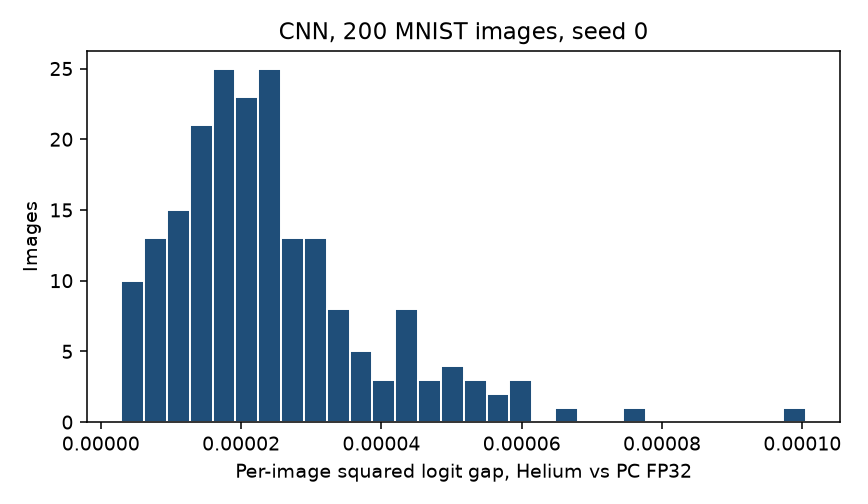
\includegraphics[width=0.78\textwidth]{helium_gap_hist.png}
\end{frame}

\begin{frame}{Cube.AI FP32 does not}
  \centering
  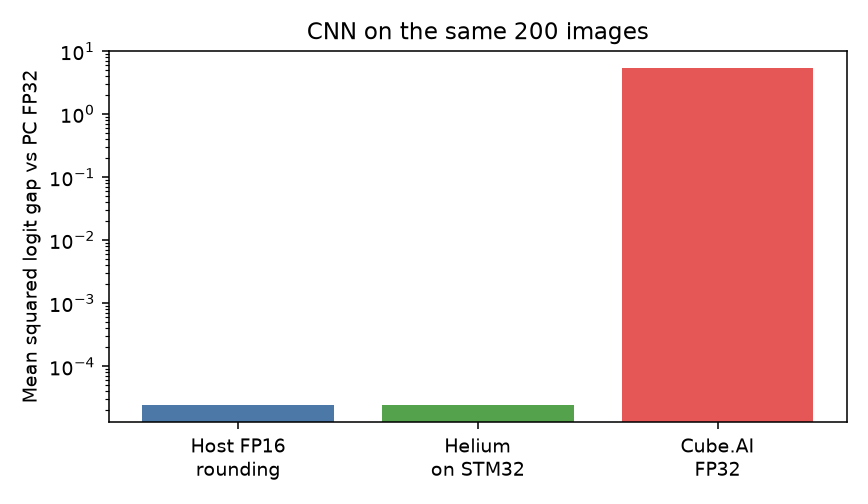
\includegraphics[width=0.78\textwidth]{mse_bars.png}

  The right-hand bar is a different compiled graph: 11 software steps and 4 accelerator steps. The class still matches.
\end{frame}

\begin{frame}{Same images, logarithmic gaps}
  \centering
  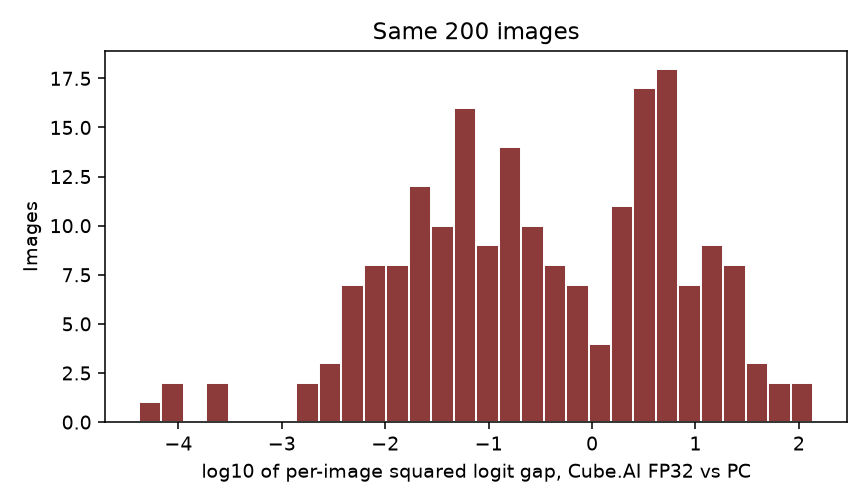
\includegraphics[width=0.72\textwidth]{cubeai_gap_hist.png}
\end{frame}

\begin{frame}{Time on the board}
  \centering
  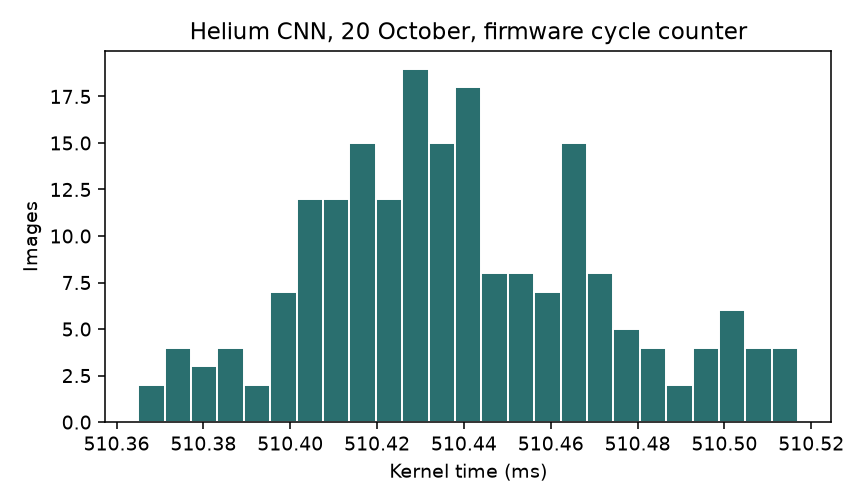
\includegraphics[width=0.72\textwidth]{latency_hist.png}

  Mean kernel time 510.4\,ms on the 20 October run. The serial transfer is not included.
\end{frame}

\begin{frame}{The same CNN, scored with \texttt{round\_fp16}}
  The checkpoint was trained for 10 epochs (best MNIST test accuracy 99.25\%).
  The Helium firmware on the board is that network: FP16 weights, FP32 activations.

  On the PC, \texttt{stm32nn.round\_fp16} cast every parameter.
  \texttt{stm32nn.compare} then scored 200 images, seed 0.

  \begin{itemize}
    \item Host, after \texttt{round\_fp16}: logit MSE \(2.422\times 10^{-5}\), class changes 0/200.
    \item Board, this morning: logit MSE \(2.422\times 10^{-5}\), class changes 0/200, 510.4\,ms.
  \end{itemize}
\end{frame}

\begin{frame}{The graded operation}
  \texttt{stm32nn.round\_fp16} is one line of PyTorch:

  \vspace{0.4em}
  \texttt{x.to(torch.float16).to(torch.float32)}

  \vspace{0.6em}
  Each finite float32 element is rounded to IEEE binary16, ties to even, and stored as float32.
  An integer tensor raises \texttt{RuntimeError} from \texttt{TORCH\_CHECK}.
\end{frame}

\begin{frame}{What \texttt{stm32nn} adds}
  A C++ PyTorch module on the PC. It does not flash the board.
  \begin{itemize}
    \item \texttt{round\_fp16}: the cast used for the matching Helium run.
    \item \texttt{to\_nhwc}, \texttt{to\_nchw}: channel-last buffers, as in the generated CNN.
    \item \texttt{quantize\_per\_channel}: symmetric int8, scale \(=\max|w|/127\).
    \item \texttt{conv2d}, \texttt{linear}, \texttt{max\_pool2d}: separate steps, optional ReLU.
    \item \texttt{compare}: MSE, class disagreement, cosine.
    \item \texttt{check\_export}: FP16 weights, a large prime channel count, pixels not divided by 255.
  \end{itemize}
\end{frame}

\begin{frame}{What the extension does not do}
  \begin{itemize}
    \item It does not replace Cube.AI's convolution.
    \item The multiply-add loop Cube.AI calls is inside a Cortex-M55 library, not in a C file we can copy.
    \item A custom ONNX operator is not compiled by ST Edge AI.
    \item The \(5.445\) gap remains until that generated graph is changed, or until the PC calls that same graph.
  \end{itemize}
\end{frame}

\begin{frame}{Tonight}
  The probe enumerated, the serial port answered, and the Helium CNN ran all 200 images.

  Result: the board and the PC rounding agree. Cube.AI's FP32 CNN, on the same images, does not agree in the logits and does agree in the class.
\end{frame}

\end{document}
